
%fitts metrics across groups, subjects and sessions
In this chapter the results processed from collected data will be presented. All data processing have been done in accordance to earlier introduced theory and implementations of methods described in \chapref{chap:Background} and \chapref{chap:Methods} respectively. The statistic results have been computed through a Friedman test, since the data proved to be non-parametric. Then a Tukey-Kramer test were done to correct for the problem of multiple comparison. All data processing have been compiled using MATLAB.


\section{Fitts' Law results} \label{sec:R:fitts}
This section will present the results acquired from the Fitts' Law target reaching test described in \secref{sec:M:fittsLaw}. The test had five metrics which each express a parameter of subjects performance. Subjects were divided into two groups, one test group which received continuous classifications scores during user training, and a control group which received binary classification scores during user training. The results have been plotted for each metric over all four sessions, with mean and standard deviations.
 

\subsection{Between test and control group}
Here the results from the Fitts' Law targets reaching test between the two groups will be presented.

%throughput
%\begin{figure}[H] 
%	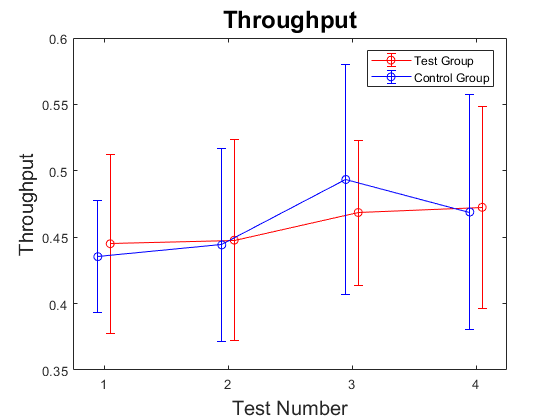
\includegraphics[width=0.4\textwidth]{figures/xWesulds/Throughput}
%	\caption{Throughput metric for the Fitts' Law test between the test and control group.}
%	\label{fig:TPresult}
%\end{figure}
%
%%Path Efficiency
%\begin{figure}[H] 
%	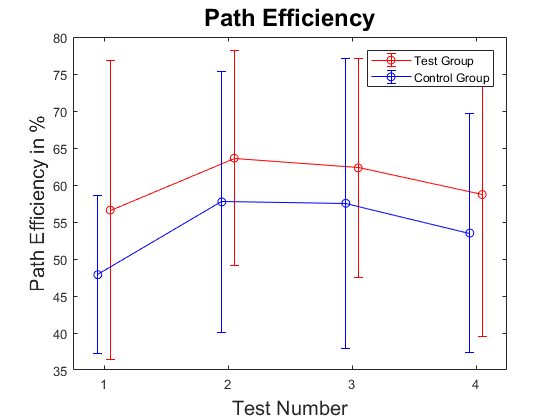
\includegraphics[width=0.4\textwidth]{figures/xWesulds/PathEfficiency}
%	\caption{Path efficiency metric for the Fitts' Law test between the test and control group.}
%	\label{fig:PEresult}
%\end{figure} 

The aim of using the Fitts' Law target reaching test were to apply a method to qualitatively evaluate the performance of subjects before, during and after completing three sessions of user training. The information drawn from the metrics are described in \secref{sub:BG:fitts}. No significant difference were found between any groups performance of any of the performance metrics ($p > 0.05$).  %throughput or path efficiency. 
%Here the subjects throughput metric inform of the subjects balance of speed and accuracy, as described in \secref{sub:BG:fitts}. Subjects path efficiency measure how well subjects

\begin{figure}[H] 
	\centering
	\subfigure[Throughput metric for the Fitts' Law test between the test and control group. There is no significant difference between the groups ($p > 0.05$).]
	{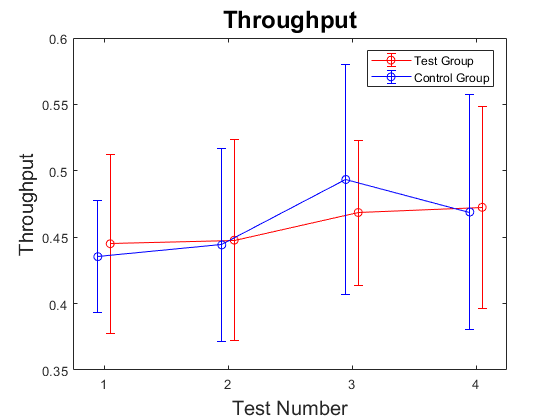
\includegraphics[width=.49\textwidth]{figures/xWesulds/Throughput}}
	\subfigure[Path efficiency metric for the Fitts' Law test between the test and control group. There is no significant difference between the groups ($p > 0.05$).]
	{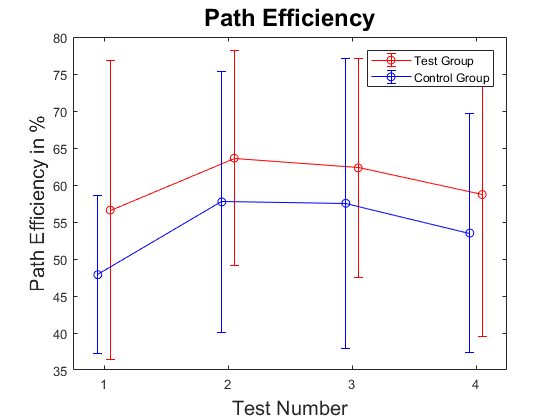
\includegraphics[width=.49\textwidth]{figures/xWesulds/PathEfficiency}}  
	\caption{Presentation of the result metrics throughput and path efficiency.}
	\label{fig:resultsTP_PE}
\end{figure}

%overshoot
%\begin{figure}[H] 
%	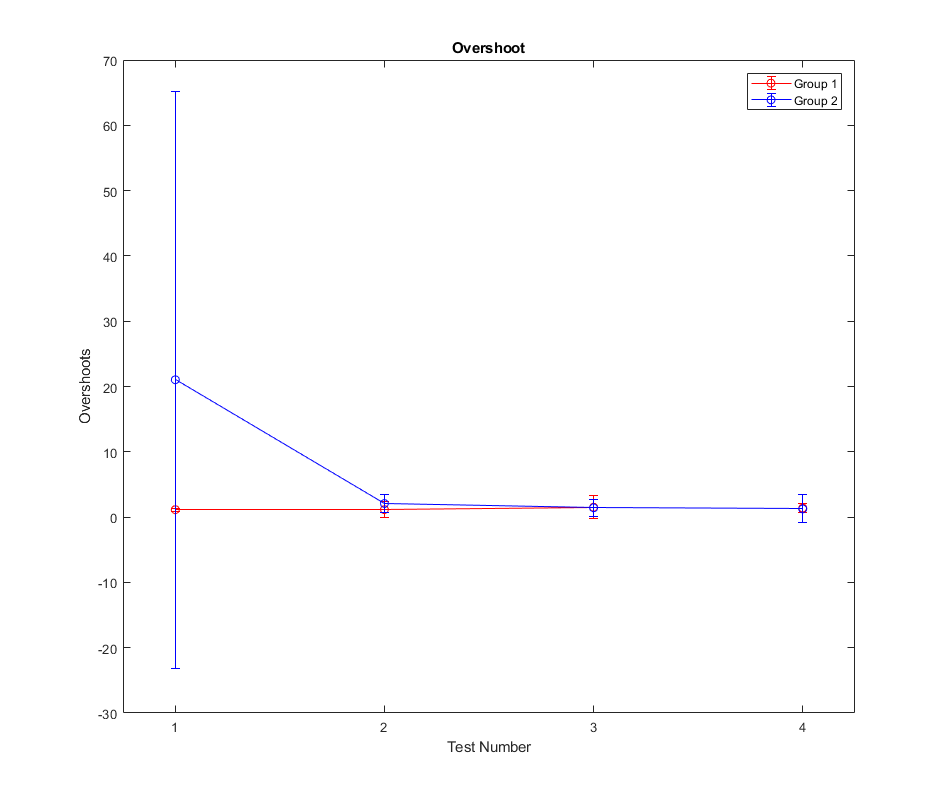
\includegraphics[width=0.4\textwidth]{figures/xWesulds/Overshoot}
%	\caption{Overshoot metric for the Fitts' Law test between the test and control group.}
%	\label{fig:OSresult}
%\end{figure} 
%
%%stopping distance
%\begin{figure}[H] 
%	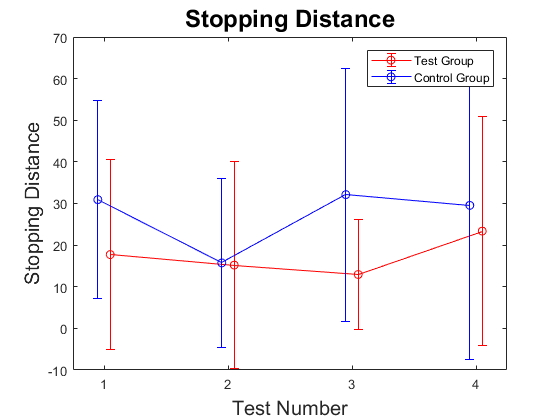
\includegraphics[width=0.4\textwidth]{figures/xWesulds/StoppingDistance}
%	\caption{Stopping distance metric for the Fitts' Law test between the test and control group.}
%	\label{fig:SDresult}
%\end{figure} 

\begin{figure}[H] 
	\centering
	\subfigure[Overshoot metric for the Fitts' Law test between the test and control group. There is no significant difference between the groups ($p > 0.05$).]
	{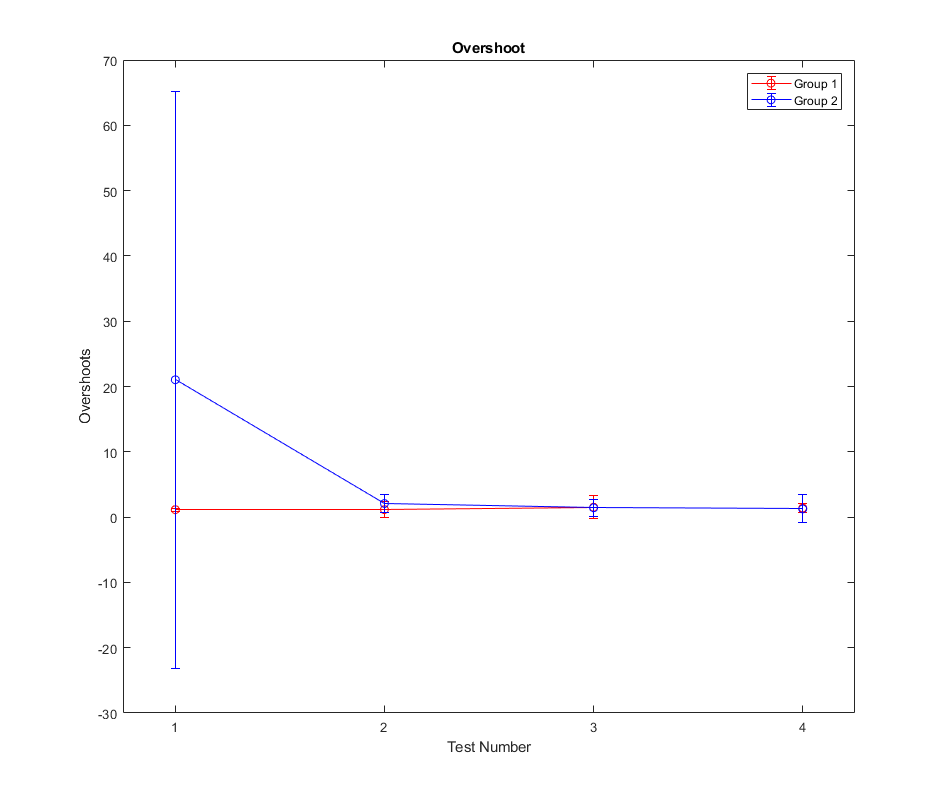
\includegraphics[width=.49\textwidth]{figures/xWesulds/Overshoot}}
	\subfigure[Stopping distance metric for the Fitts' Law test between the test and control group. There is no significant difference between the groups ($p > 0.05$).]
	{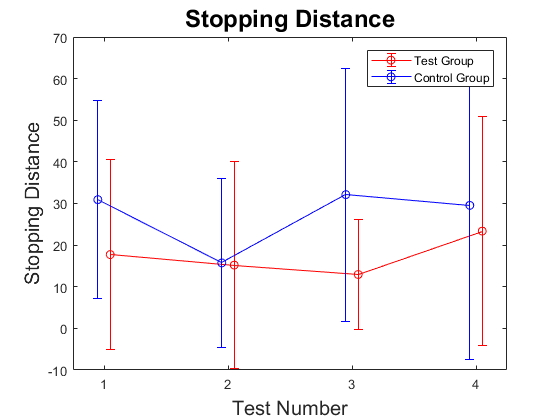
\includegraphics[width=.49\textwidth]{figures/xWesulds/StoppingDistance}}  
	\caption{Presentation of the result metrics overshoot and stopping distance.}
	\label{fig:resultsOS_SD}
\end{figure}

%completion rate
\begin{figure}[H] 
	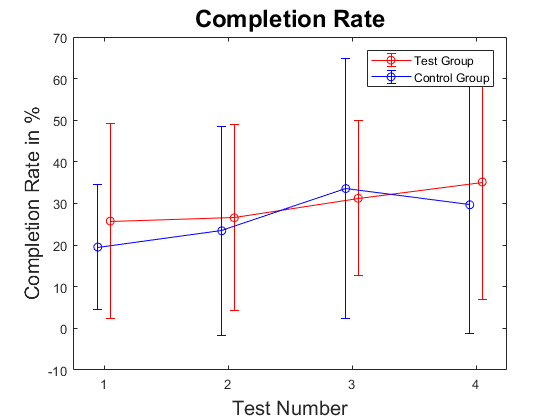
\includegraphics[width=0.49\textwidth]{figures/xWesulds/CompletionRate}
	\caption{Completion rate metric for the Fitts' Law test between the test and control group. There is no significant difference between the groups ($p > 0.05$).}
	\label{fig:CRresult}
\end{figure} 


\subsection{Across sessions}

No significant difference in performance was found between the four tests with $p > 0.05$ for both the overall Friedmans test and the Tukey-Kramer correction to test difference between each session. This was the case for both the test and control group, which means there was no significant development of performance between either of the sessions for any group.

